\documentclass[1p]{elsarticle_modified}
%\bibliographystyle{elsarticle-num}

%\usepackage[colorlinks]{hyperref}
%\usepackage{abbrmath_seonhwa} %\Abb, \Ascr, \Acal ,\Abf, \Afrak
\usepackage{amsfonts}
\usepackage{amssymb}
\usepackage{amsmath}
\usepackage{amsthm}
\usepackage{scalefnt}
\usepackage{amsbsy}
\usepackage{kotex}
\usepackage{caption}
\usepackage{subfig}
\usepackage{color}
\usepackage{graphicx}
\usepackage{xcolor} %% white, black, red, green, blue, cyan, magenta, yellow
\usepackage{float}
\usepackage{setspace}
\usepackage{hyperref}

\usepackage{tikz}
\usetikzlibrary{arrows}

\usepackage{multirow}
\usepackage{array} % fixed length table
\usepackage{hhline}

%%%%%%%%%%%%%%%%%%%%%
\makeatletter
\renewcommand*\env@matrix[1][\arraystretch]{%
	\edef\arraystretch{#1}%
	\hskip -\arraycolsep
	\let\@ifnextchar\new@ifnextchar
	\array{*\c@MaxMatrixCols c}}
\makeatother %https://tex.stackexchange.com/questions/14071/how-can-i-increase-the-line-spacing-in-a-matrix
%%%%%%%%%%%%%%%

\usepackage[normalem]{ulem}

\newcommand{\msout}[1]{\ifmmode\text{\sout{\ensuremath{#1}}}\else\sout{#1}\fi}
%SOURCE: \msout is \stkout macro in https://tex.stackexchange.com/questions/20609/strikeout-in-math-mode

\newcommand{\cancel}[1]{
	\ifmmode
	{\color{red}\msout{#1}}
	\else
	{\color{red}\sout{#1}}
	\fi
}

\newcommand{\add}[1]{
	{\color{blue}\uwave{#1}}
}

\newcommand{\replace}[2]{
	\ifmmode
	{\color{red}\msout{#1}}{\color{blue}\uwave{#2}}
	\else
	{\color{red}\sout{#1}}{\color{blue}\uwave{#2}}
	\fi
}

\newcommand{\Sol}{\mathcal{S}} %segment
\newcommand{\D}{D} %diagram
\newcommand{\A}{\mathcal{A}} %arc


%%%%%%%%%%%%%%%%%%%%%%%%%%%%%5 test

\def\sl{\operatorname{\textup{SL}}(2,\Cbb)}
\def\psl{\operatorname{\textup{PSL}}(2,\Cbb)}
\def\quan{\mkern 1mu \triangleright \mkern 1mu}

\theoremstyle{definition}
\newtheorem{thm}{Theorem}[section]
\newtheorem{prop}[thm]{Proposition}
\newtheorem{lem}[thm]{Lemma}
\newtheorem{ques}[thm]{Question}
\newtheorem{cor}[thm]{Corollary}
\newtheorem{defn}[thm]{Definition}
\newtheorem{exam}[thm]{Example}
\newtheorem{rmk}[thm]{Remark}
\newtheorem{alg}[thm]{Algorithm}

\newcommand{\I}{\sqrt{-1}}
\begin{document}

%\begin{frontmatter}
%
%\title{Boundary parabolic representations of knots up to 8 crossings}
%
%%% Group authors per affiliation:
%\author{Yunhi Cho} 
%\address{Department of Mathematics, University of Seoul, Seoul, Korea}
%\ead{yhcho@uos.ac.kr}
%
%
%\author{Seonhwa Kim} %\fnref{s_kim}}
%\address{Center for Geometry and Physics, Institute for Basic Science, Pohang, 37673, Korea}
%\ead{ryeona17@ibs.re.kr}
%
%\author{Hyuk Kim}
%\address{Department of Mathematical Sciences, Seoul National University, Seoul 08826, Korea}
%\ead{hyukkim@snu.ac.kr}
%
%\author{Seokbeom Yoon}
%\address{Department of Mathematical Sciences, Seoul National University, Seoul, 08826,  Korea}
%\ead{sbyoon15@snu.ac.kr}
%
%\begin{abstract}
%We find all boundary parabolic representation of knots up to 8 crossings.
%
%\end{abstract}
%\begin{keyword}
%    \MSC[2010] 57M25 
%\end{keyword}
%
%\end{frontmatter}

%\linenumbers
%\tableofcontents
%
\newcommand\colored[1]{\textcolor{white}{\rule[-0.35ex]{0.8em}{1.4ex}}\kern-0.8em\color{red} #1}%
%\newcommand\colored[1]{\textcolor{white}{ #1}\kern-2.17ex	\textcolor{white}{ #1}\kern-1.81ex	\textcolor{white}{ #1}\kern-2.15ex\color{red}#1	}

{\Large $\underline{12n_{0846}~(K12n_{0846})}$}

\setlength{\tabcolsep}{10pt}
\renewcommand{\arraystretch}{1.6}
\vspace{1cm}\begin{tabular}{m{100pt}>{\centering\arraybackslash}m{274pt}}
\multirow{5}{120pt}{
	\centering
	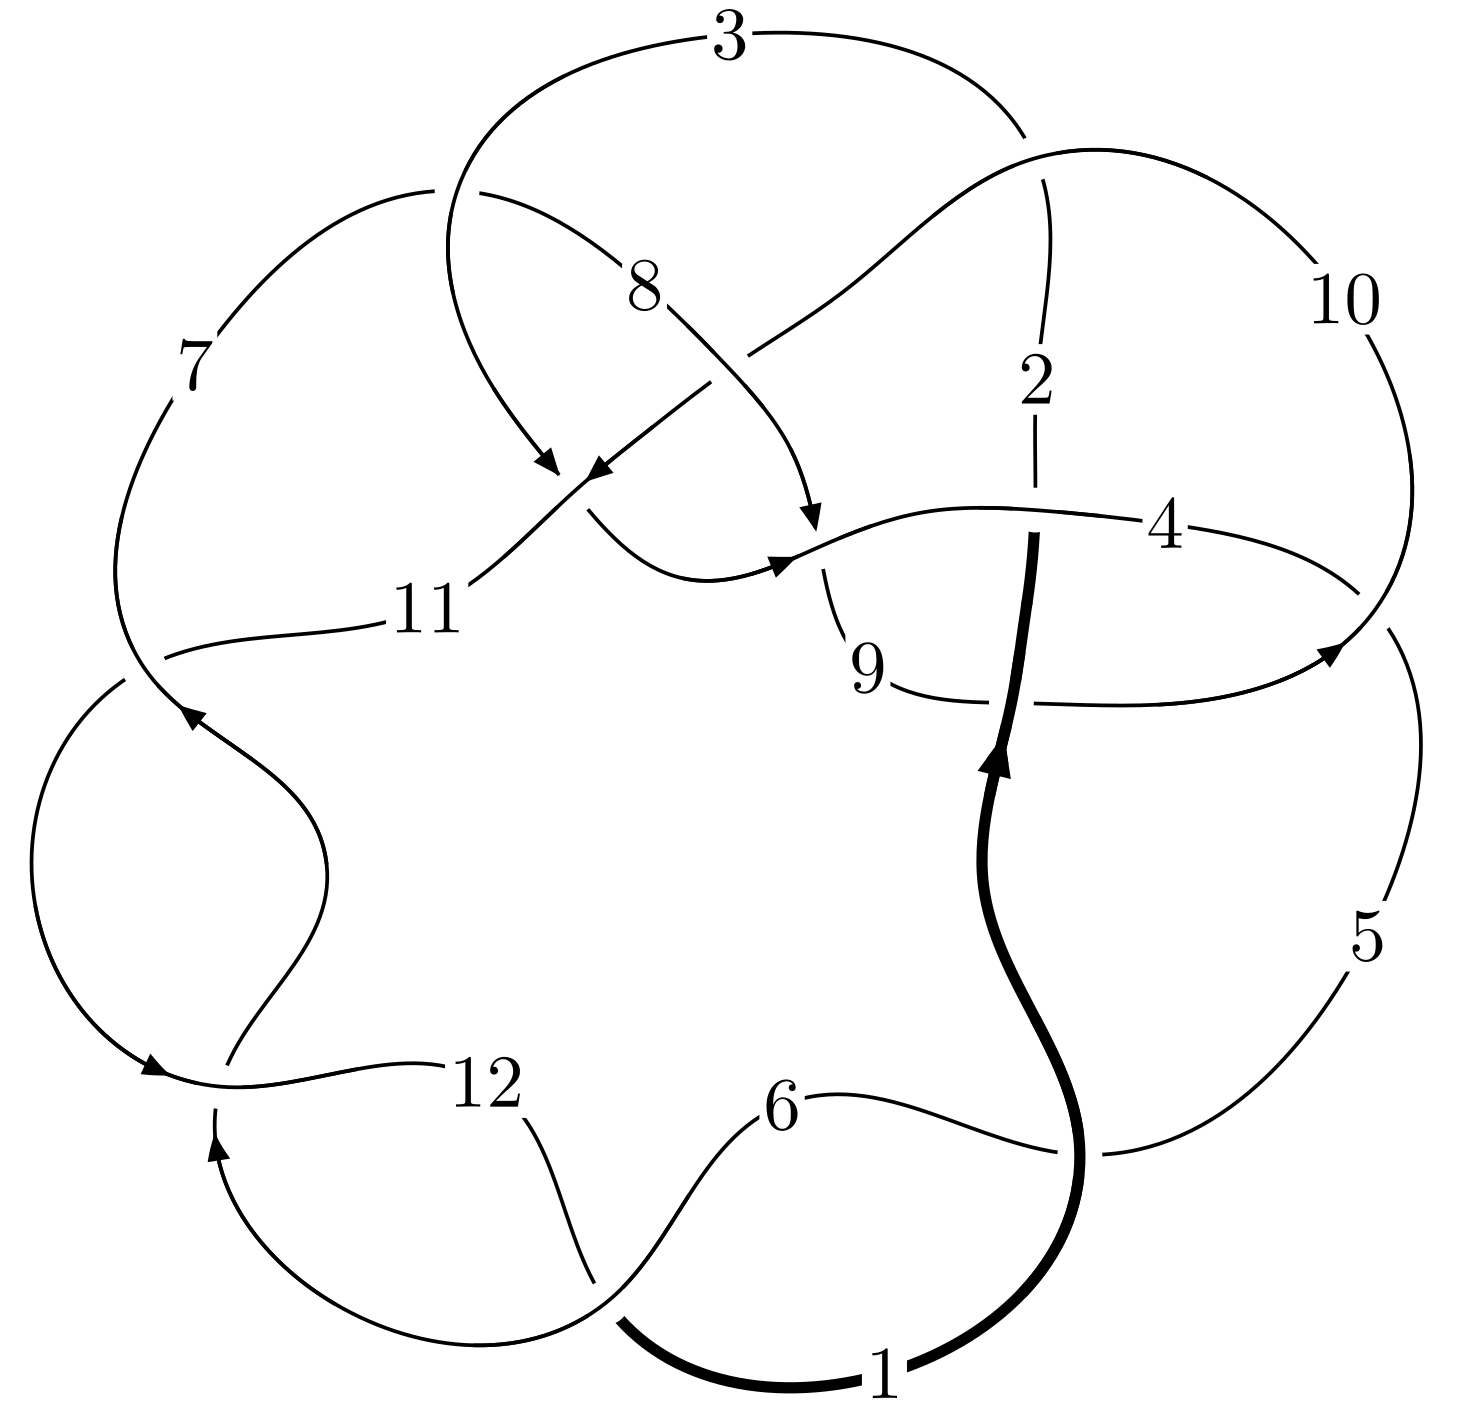
\includegraphics[width=112pt]{../../../GIT/diagram.site/Diagrams/png/2935_12n_0846.png}\\
\ \ \ A knot diagram\footnotemark}&
\allowdisplaybreaks
\textbf{Linearized knot diagam} \\
\cline{2-2}
 &
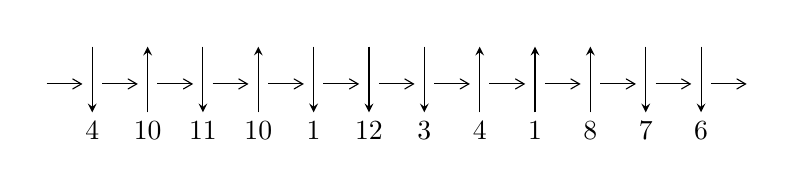
\begin{tikzpicture}[x=20pt, y=17pt]
	% nodes
	\node (C0) at (0, 0) {};
	\node (C1) at (1, 0) {};
	\node (C1U) at (1, +1) {};
	\node (C1D) at (1, -1) {4};

	\node (C2) at (2, 0) {};
	\node (C2U) at (2, +1) {};
	\node (C2D) at (2, -1) {10};

	\node (C3) at (3, 0) {};
	\node (C3U) at (3, +1) {};
	\node (C3D) at (3, -1) {11};

	\node (C4) at (4, 0) {};
	\node (C4U) at (4, +1) {};
	\node (C4D) at (4, -1) {10};

	\node (C5) at (5, 0) {};
	\node (C5U) at (5, +1) {};
	\node (C5D) at (5, -1) {1};

	\node (C6) at (6, 0) {};
	\node (C6U) at (6, +1) {};
	\node (C6D) at (6, -1) {12};

	\node (C7) at (7, 0) {};
	\node (C7U) at (7, +1) {};
	\node (C7D) at (7, -1) {3};

	\node (C8) at (8, 0) {};
	\node (C8U) at (8, +1) {};
	\node (C8D) at (8, -1) {4};

	\node (C9) at (9, 0) {};
	\node (C9U) at (9, +1) {};
	\node (C9D) at (9, -1) {1};

	\node (C10) at (10, 0) {};
	\node (C10U) at (10, +1) {};
	\node (C10D) at (10, -1) {8};

	\node (C11) at (11, 0) {};
	\node (C11U) at (11, +1) {};
	\node (C11D) at (11, -1) {7};

	\node (C12) at (12, 0) {};
	\node (C12U) at (12, +1) {};
	\node (C12D) at (12, -1) {6};
	\node (C13) at (13, 0) {};

	% arrows
	\draw[->,>={angle 60}]
	(C0) edge (C1) (C1) edge (C2) (C2) edge (C3) (C3) edge (C4) (C4) edge (C5) (C5) edge (C6) (C6) edge (C7) (C7) edge (C8) (C8) edge (C9) (C9) edge (C10) (C10) edge (C11) (C11) edge (C12) (C12) edge (C13) ;	\draw[->,>=stealth]
	(C1U) edge (C1D) (C2D) edge (C2U) (C3U) edge (C3D) (C4D) edge (C4U) (C5U) edge (C5D) (C6U) edge (C6D) (C7U) edge (C7D) (C8D) edge (C8U) (C9D) edge (C9U) (C10D) edge (C10U) (C11U) edge (C11D) (C12U) edge (C12D) ;
	\end{tikzpicture} \\
\hhline{~~} \\& 
\textbf{Solving Sequence} \\ \cline{2-2} 
 &
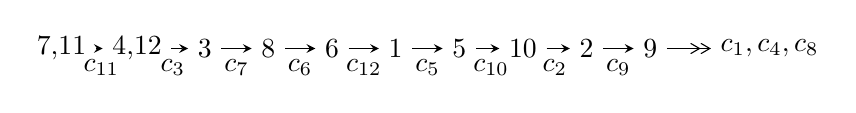
\begin{tikzpicture}[x=23pt, y=7pt]
	% node
	\node (A0) at (-1/8, 0) {7,11};
	\node (A1) at (17/16, 0) {4,12};
	\node (A2) at (17/8, 0) {3};
	\node (A3) at (25/8, 0) {8};
	\node (A4) at (33/8, 0) {6};
	\node (A5) at (41/8, 0) {1};
	\node (A6) at (49/8, 0) {5};
	\node (A7) at (57/8, 0) {10};
	\node (A8) at (65/8, 0) {2};
	\node (A9) at (73/8, 0) {9};
	\node (C1) at (1/2, -1) {$c_{11}$};
	\node (C2) at (13/8, -1) {$c_{3}$};
	\node (C3) at (21/8, -1) {$c_{7}$};
	\node (C4) at (29/8, -1) {$c_{6}$};
	\node (C5) at (37/8, -1) {$c_{12}$};
	\node (C6) at (45/8, -1) {$c_{5}$};
	\node (C7) at (53/8, -1) {$c_{10}$};
	\node (C8) at (61/8, -1) {$c_{2}$};
	\node (C9) at (69/8, -1) {$c_{9}$};
	\node (A10) at (11, 0) {$c_{1},c_{4},c_{8}$};

	% edge
	\draw[->,>=stealth]	
	(A0) edge (A1) (A1) edge (A2) (A2) edge (A3) (A3) edge (A4) (A4) edge (A5) (A5) edge (A6) (A6) edge (A7) (A7) edge (A8) (A8) edge (A9) ;
	\draw[->>,>={angle 60}]	
	(A9) edge (A10);
\end{tikzpicture} \\ 

\end{tabular} \\

\footnotetext{
The image of knot diagram is generated by the software ``\textbf{Draw programme}" developed by Andrew Bartholomew(\url{http://www.layer8.co.uk/maths/draw/index.htm\#Running-draw}), where we modified some parts for our purpose(\url{https://github.com/CATsTAILs/LinksPainter}).
}\phantom \\ \newline 
\centering \textbf{Ideals for irreducible components\footnotemark of $X_{\text{par}}$} 
 
\begin{align*}
I^u_{1}&=\langle 
-5 u^{21}+43 u^{20}+\cdots+8 b+200,\;-15 u^{21}+129 u^{20}+\cdots+16 a+272,\;u^{22}-9 u^{21}+\cdots-176 u+16\rangle \\
I^u_{2}&=\langle 
u^3 a- u^3+3 a u-2 u^2+2 b+a-3 u-5,\;3 u^3 a+2 u^2 a+u^3+a^2+8 a u-2 u^2+3 a+2 u-2,\\
\phantom{I^u_{2}}&\phantom{= \langle  }u^4+u^3+3 u^2+2 u+1\rangle \\
I^u_{3}&=\langle 
u^{10}+7 u^8+17 u^6- u^5+17 u^4-2 u^3+7 u^2+b+u+1,\\
\phantom{I^u_{3}}&\phantom{= \langle  }- u^{13}-10 u^{11}-2 u^{10}-37 u^9-13 u^8-61 u^7-29 u^6-39 u^5-30 u^4- u^3-19 u^2+2 a+2 u-1,\\
\phantom{I^u_{3}}&\phantom{= \langle  }u^{14}+10 u^{12}+39 u^{10}- u^9+75 u^8-5 u^7+75 u^6-6 u^5+39 u^4+u^3+10 u^2+u+2\rangle \\
I^u_{4}&=\langle 
64742 a^5 u^3+484970 a^4 u^3+\cdots-385898 a-56434,\;3 a^5 u^3-2 a^4 u^3+\cdots+8 a-9,\\
\phantom{I^u_{4}}&\phantom{= \langle  }u^4+u^3+3 u^2+2 u+1\rangle \\
\\
\end{align*}
\raggedright * 4 irreducible components of $\dim_{\mathbb{C}}=0$, with total 68 representations.\\
\footnotetext{All coefficients of polynomials are rational numbers. But the coefficients are sometimes approximated in decimal forms when there is not enough margin.}
\newpage
\renewcommand{\arraystretch}{1}
\centering \section*{I. $I^u_{1}= \langle -5 u^{21}+43 u^{20}+\cdots+8 b+200,\;-15 u^{21}+129 u^{20}+\cdots+16 a+272,\;u^{22}-9 u^{21}+\cdots-176 u+16 \rangle$}
\flushleft \textbf{(i) Arc colorings}\\
\begin{tabular}{m{7pt} m{180pt} m{7pt} m{180pt} }
\flushright $a_{7}=$&$\begin{pmatrix}0\\u\end{pmatrix}$ \\
\flushright $a_{11}=$&$\begin{pmatrix}1\\0\end{pmatrix}$ \\
\flushright $a_{4}=$&$\begin{pmatrix}\frac{15}{16} u^{21}-\frac{129}{16} u^{20}+\cdots+\frac{359}{2} u-17\\\frac{5}{8} u^{21}-\frac{43}{8} u^{20}+\cdots+233 u-25\end{pmatrix}$ \\
\flushright $a_{12}=$&$\begin{pmatrix}1\\u^2\end{pmatrix}$ \\
\flushright $a_{3}=$&$\begin{pmatrix}\frac{25}{16} u^{21}-\frac{215}{16} u^{20}+\cdots+\frac{825}{2} u-42\\\frac{5}{8} u^{21}-\frac{43}{8} u^{20}+\cdots+233 u-25\end{pmatrix}$ \\
\flushright $a_{8}=$&$\begin{pmatrix}-1.37500 u^{21}+11.2500 u^{20}+\cdots-398.750 u+45.5000\\-\frac{9}{8} u^{21}+\frac{73}{8} u^{20}+\cdots-\frac{391}{2} u+22\end{pmatrix}$ \\
\flushright $a_{6}=$&$\begin{pmatrix}u\\u^3+u\end{pmatrix}$ \\
\flushright $a_{1}=$&$\begin{pmatrix}u^2+1\\u^4+2 u^2\end{pmatrix}$ \\
\flushright $a_{5}=$&$\begin{pmatrix}u^3+2 u\\u^5+3 u^3+u\end{pmatrix}$ \\
\flushright $a_{10}=$&$\begin{pmatrix}0.812500 u^{21}-6.81250 u^{20}+\cdots+76.7500 u-6.50000\\-\frac{1}{2} u^{21}+\frac{15}{4} u^{20}+\cdots-\frac{81}{2} u+5\end{pmatrix}$ \\
\flushright $a_{2}=$&$\begin{pmatrix}u^{21}-\frac{67}{8} u^{20}+\cdots+\frac{837}{4} u-\frac{41}{2}\\\frac{5}{8} u^{21}-\frac{45}{8} u^{20}+\cdots+\frac{477}{2} u-26\end{pmatrix}$ \\
\flushright $a_{9}=$&$\begin{pmatrix}0.812500 u^{21}-7.06250 u^{20}+\cdots+255.250 u-27.5000\\-\frac{1}{2} u^{21}+\frac{19}{4} u^{20}+\cdots-\frac{273}{2} u+13\end{pmatrix}$\\&\end{tabular}
\flushleft \textbf{(ii) Obstruction class $= -1$}\\~\\
\flushleft \textbf{(iii) Cusp Shapes $= \frac{1}{2} u^{21}-\frac{9}{2} u^{20}+\frac{53}{2} u^{19}-114 u^{18}+395 u^{17}-1141 u^{16}+\frac{5639}{2} u^{15}-\frac{12093}{2} u^{14}+11359 u^{13}-\frac{37595}{2} u^{12}+\frac{54937}{2} u^{11}-\frac{70905}{2} u^{10}+\frac{80651}{2} u^9-40255 u^8+35027 u^7-26326 u^6+16866 u^5-\frac{18113}{2} u^4+3971 u^3-1368 u^2+346 u-54$}\\~\\
\newpage\renewcommand{\arraystretch}{1}
\flushleft \textbf{(iv) u-Polynomials at the component}\newline \\
\begin{tabular}{m{50pt}|m{274pt}}
Crossings & \hspace{64pt}u-Polynomials at each crossing \\
\hline $$\begin{aligned}c_{1}\end{aligned}$$&$\begin{aligned}
&u^{22}-19 u^{21}+\cdots-640 u+256
\end{aligned}$\\
\hline $$\begin{aligned}c_{2},c_{8}\end{aligned}$$&$\begin{aligned}
&u^{22}+u^{21}+\cdots-2 u+2
\end{aligned}$\\
\hline $$\begin{aligned}c_{3},c_{7}\end{aligned}$$&$\begin{aligned}
&u^{22}+3 u^{20}+\cdots- u^2+1
\end{aligned}$\\
\hline $$\begin{aligned}c_{4},c_{9}\end{aligned}$$&$\begin{aligned}
&u^{22}+14 u^{20}+\cdots+u+1
\end{aligned}$\\
\hline $$\begin{aligned}c_{5},c_{6},c_{11}\\c_{12}\end{aligned}$$&$\begin{aligned}
&u^{22}+9 u^{21}+\cdots+176 u+16
\end{aligned}$\\
\hline $$\begin{aligned}c_{10}\end{aligned}$$&$\begin{aligned}
&u^{22}+15 u^{21}+\cdots+160 u+16
\end{aligned}$\\
\hline
\end{tabular}\\~\\
\newpage\renewcommand{\arraystretch}{1}
\flushleft \textbf{(v) Riley Polynomials at the component}\newline \\
\begin{tabular}{m{50pt}|m{274pt}}
Crossings & \hspace{64pt}Riley Polynomials at each crossing \\
\hline $$\begin{aligned}c_{1}\end{aligned}$$&$\begin{aligned}
&y^{22}-17 y^{21}+\cdots+483328 y+65536
\end{aligned}$\\
\hline $$\begin{aligned}c_{2},c_{8}\end{aligned}$$&$\begin{aligned}
&y^{22}+3 y^{21}+\cdots+32 y+4
\end{aligned}$\\
\hline $$\begin{aligned}c_{3},c_{7}\end{aligned}$$&$\begin{aligned}
&y^{22}+6 y^{21}+\cdots-2 y+1
\end{aligned}$\\
\hline $$\begin{aligned}c_{4},c_{9}\end{aligned}$$&$\begin{aligned}
&y^{22}+28 y^{21}+\cdots+11 y+1
\end{aligned}$\\
\hline $$\begin{aligned}c_{5},c_{6},c_{11}\\c_{12}\end{aligned}$$&$\begin{aligned}
&y^{22}+25 y^{21}+\cdots-384 y+256
\end{aligned}$\\
\hline $$\begin{aligned}c_{10}\end{aligned}$$&$\begin{aligned}
&y^{22}+7 y^{21}+\cdots+2432 y+256
\end{aligned}$\\
\hline
\end{tabular}\\~\\
\newpage\flushleft \textbf{(vi) Complex Volumes and Cusp Shapes}
$$\begin{array}{c|c|c}  
\text{Solutions to }I^u_{1}& \I (\text{vol} + \sqrt{-1}CS) & \text{Cusp shape}\\
 \hline 
\begin{aligned}
u &= \phantom{-}0.287964 + 0.924780 I \\
a &= -0.34728 + 1.43125 I \\
b &= -0.805889 - 0.918892 I\end{aligned}
 & \phantom{-}2.14244 - 3.29575 I & -1.06475 + 2.74337 I \\ \hline\begin{aligned}
u &= \phantom{-}0.287964 - 0.924780 I \\
a &= -0.34728 - 1.43125 I \\
b &= -0.805889 + 0.918892 I\end{aligned}
 & \phantom{-}2.14244 + 3.29575 I & -1.06475 - 2.74337 I \\ \hline\begin{aligned}
u &= \phantom{-}0.927630 + 0.184659 I \\
a &= \phantom{-}0.129761 + 0.188778 I \\
b &= -0.777225 + 0.767673 I\end{aligned}
 & -6.83184 + 5.48292 I & -4.03618 - 4.85229 I \\ \hline\begin{aligned}
u &= \phantom{-}0.927630 - 0.184659 I \\
a &= \phantom{-}0.129761 - 0.188778 I \\
b &= -0.777225 - 0.767673 I\end{aligned}
 & -6.83184 - 5.48292 I & -4.03618 + 4.85229 I \\ \hline\begin{aligned}
u &= \phantom{-}0.842891 + 0.639931 I \\
a &= \phantom{-}0.429405 - 0.313332 I \\
b &= \phantom{-}0.187769 + 0.832828 I\end{aligned}
 & -2.36000 - 2.86683 I & \phantom{-}3.02711 + 5.17659 I \\ \hline\begin{aligned}
u &= \phantom{-}0.842891 - 0.639931 I \\
a &= \phantom{-}0.429405 + 0.313332 I \\
b &= \phantom{-}0.187769 - 0.832828 I\end{aligned}
 & -2.36000 + 2.86683 I & \phantom{-}3.02711 - 5.17659 I \\ \hline\begin{aligned}
u &= \phantom{-}0.702570 + 0.819082 I \\
a &= \phantom{-}0.363866 - 1.106770 I \\
b &= \phantom{-}0.97246 + 1.06574 I\end{aligned}
 & -4.90801 - 10.80840 I & -1.85897 + 7.63550 I \\ \hline\begin{aligned}
u &= \phantom{-}0.702570 - 0.819082 I \\
a &= \phantom{-}0.363866 + 1.106770 I \\
b &= \phantom{-}0.97246 - 1.06574 I\end{aligned}
 & -4.90801 + 10.80840 I & -1.85897 - 7.63550 I \\ \hline\begin{aligned}
u &= \phantom{-}0.117025 + 0.707443 I \\
a &= \phantom{-}0.327460 + 0.729010 I \\
b &= -0.504470 - 0.045202 I\end{aligned}
 & \phantom{-}0.65660 - 1.39506 I & \phantom{-}0.82058 + 5.90353 I \\ \hline\begin{aligned}
u &= \phantom{-}0.117025 - 0.707443 I \\
a &= \phantom{-}0.327460 - 0.729010 I \\
b &= -0.504470 + 0.045202 I\end{aligned}
 & \phantom{-}0.65660 + 1.39506 I & \phantom{-}0.82058 - 5.90353 I\\
 \hline 
 \end{array}$$\newpage$$\begin{array}{c|c|c}  
\text{Solutions to }I^u_{1}& \I (\text{vol} + \sqrt{-1}CS) & \text{Cusp shape}\\
 \hline 
\begin{aligned}
u &= \phantom{-}0.59656 + 1.29686 I \\
a &= -0.600773 + 0.160192 I \\
b &= \phantom{-}0.356754 - 0.547531 I\end{aligned}
 & -2.42718 + 0.16938 I & \phantom{-}2.49026 - 5.93197 I \\ \hline\begin{aligned}
u &= \phantom{-}0.59656 - 1.29686 I \\
a &= -0.600773 - 0.160192 I \\
b &= \phantom{-}0.356754 + 0.547531 I\end{aligned}
 & -2.42718 - 0.16938 I & \phantom{-}2.49026 + 5.93197 I \\ \hline\begin{aligned}
u &= \phantom{-}0.454810 + 0.112434 I \\
a &= \phantom{-}0.910049 + 0.178219 I \\
b &= \phantom{-}0.626422 + 0.465538 I\end{aligned}
 & -1.041380 - 0.734179 I & -6.66165 + 2.13353 I \\ \hline\begin{aligned}
u &= \phantom{-}0.454810 - 0.112434 I \\
a &= \phantom{-}0.910049 - 0.178219 I \\
b &= \phantom{-}0.626422 - 0.465538 I\end{aligned}
 & -1.041380 + 0.734179 I & -6.66165 - 2.13353 I \\ \hline\begin{aligned}
u &= \phantom{-}0.25923 + 1.61438 I \\
a &= -0.255394 + 1.262780 I \\
b &= -0.450728 - 1.096960 I\end{aligned}
 & \phantom{-}5.16479 - 6.92628 I & \phantom{-}2.76500 + 4.70851 I \\ \hline\begin{aligned}
u &= \phantom{-}0.25923 - 1.61438 I \\
a &= -0.255394 - 1.262780 I \\
b &= -0.450728 + 1.096960 I\end{aligned}
 & \phantom{-}5.16479 + 6.92628 I & \phantom{-}2.76500 - 4.70851 I \\ \hline\begin{aligned}
u &= \phantom{-}0.22193 + 1.65185 I \\
a &= \phantom{-}0.18340 + 1.86093 I \\
b &= -1.06261 - 1.33577 I\end{aligned}
 & \phantom{-}3.3965 - 14.3712 I & \phantom{-}0.70200 + 6.98452 I \\ \hline\begin{aligned}
u &= \phantom{-}0.22193 - 1.65185 I \\
a &= \phantom{-}0.18340 - 1.86093 I \\
b &= -1.06261 + 1.33577 I\end{aligned}
 & \phantom{-}3.3965 + 14.3712 I & \phantom{-}0.70200 - 6.98452 I \\ \hline\begin{aligned}
u &= \phantom{-}0.07299 + 1.69387 I \\
a &= -0.25150 - 1.73742 I \\
b &= \phantom{-}0.97828 + 1.19120 I\end{aligned}
 & \phantom{-}11.37540 - 4.70341 I & -1.53492 - 1.20569 I \\ \hline\begin{aligned}
u &= \phantom{-}0.07299 - 1.69387 I \\
a &= -0.25150 + 1.73742 I \\
b &= \phantom{-}0.97828 - 1.19120 I\end{aligned}
 & \phantom{-}11.37540 + 4.70341 I & -1.53492 + 1.20569 I\\
 \hline 
 \end{array}$$\newpage$$\begin{array}{c|c|c}  
\text{Solutions to }I^u_{1}& \I (\text{vol} + \sqrt{-1}CS) & \text{Cusp shape}\\
 \hline 
\begin{aligned}
u &= \phantom{-}0.01640 + 1.72547 I \\
a &= -0.138986 - 0.857092 I \\
b &= \phantom{-}0.479233 + 0.582586 I\end{aligned}
 & \phantom{-}9.63715 - 1.43342 I & \phantom{-}1.85153 + 4.64223 I \\ \hline\begin{aligned}
u &= \phantom{-}0.01640 - 1.72547 I \\
a &= -0.138986 + 0.857092 I \\
b &= \phantom{-}0.479233 - 0.582586 I\end{aligned}
 & \phantom{-}9.63715 + 1.43342 I & \phantom{-}1.85153 - 4.64223 I\\
 \hline 
 \end{array}$$\newpage\newpage\renewcommand{\arraystretch}{1}
\centering \section*{II. $I^u_{2}= \langle u^3 a- u^3+3 a u-2 u^2+2 b+a-3 u-5,\;3 u^3 a+u^3+\cdots+3 a-2,\;u^4+u^3+3 u^2+2 u+1 \rangle$}
\flushleft \textbf{(i) Arc colorings}\\
\begin{tabular}{m{7pt} m{180pt} m{7pt} m{180pt} }
\flushright $a_{7}=$&$\begin{pmatrix}0\\u\end{pmatrix}$ \\
\flushright $a_{11}=$&$\begin{pmatrix}1\\0\end{pmatrix}$ \\
\flushright $a_{4}=$&$\begin{pmatrix}a\\-\frac{1}{2} u^3 a+\frac{1}{2} u^3+\cdots-\frac{1}{2} a+\frac{5}{2}\end{pmatrix}$ \\
\flushright $a_{12}=$&$\begin{pmatrix}1\\u^2\end{pmatrix}$ \\
\flushright $a_{3}=$&$\begin{pmatrix}-\frac{1}{2} u^3 a+\frac{1}{2} u^3+\cdots+\frac{1}{2} a+\frac{5}{2}\\-\frac{1}{2} u^3 a+\frac{1}{2} u^3+\cdots-\frac{1}{2} a+\frac{5}{2}\end{pmatrix}$ \\
\flushright $a_{8}=$&$\begin{pmatrix}-\frac{1}{2} u^3 a-\frac{3}{2} u^3+\cdots-\frac{5}{2} a-\frac{5}{2}\\u^3+u^2+2 u+1\end{pmatrix}$ \\
\flushright $a_{6}=$&$\begin{pmatrix}u\\u^3+u\end{pmatrix}$ \\
\flushright $a_{1}=$&$\begin{pmatrix}u^2+1\\- u^3- u^2-2 u-1\end{pmatrix}$ \\
\flushright $a_{5}=$&$\begin{pmatrix}u^3+2 u\\u^3+u^2+2 u+1\end{pmatrix}$ \\
\flushright $a_{10}=$&$\begin{pmatrix}-\frac{3}{2} u^3 a-\frac{1}{2} u^3+\cdots-\frac{3}{2} a+\frac{3}{2}\\u\end{pmatrix}$ \\
\flushright $a_{2}=$&$\begin{pmatrix}u^2 a+u^2+2 a+1\\-\frac{3}{2} u^3 a-\frac{1}{2} u^3+\cdots-\frac{3}{2} a+\frac{7}{2}\end{pmatrix}$ \\
\flushright $a_{9}=$&$\begin{pmatrix}-\frac{1}{2} u^3 a-\frac{3}{2} u^3+\cdots-\frac{3}{2} a-\frac{3}{2}\\\frac{1}{2} u^3 a+\frac{3}{2} u^3+\cdots+\frac{3}{2} a+\frac{1}{2}\end{pmatrix}$\\&\end{tabular}
\flushleft \textbf{(ii) Obstruction class $= -1$}\\~\\
\flushleft \textbf{(iii) Cusp Shapes $= -8 u^3-8 u^2-24 u-14$}\\~\\
\newpage\renewcommand{\arraystretch}{1}
\flushleft \textbf{(iv) u-Polynomials at the component}\newline \\
\begin{tabular}{m{50pt}|m{274pt}}
Crossings & \hspace{64pt}u-Polynomials at each crossing \\
\hline $$\begin{aligned}c_{1}\end{aligned}$$&$\begin{aligned}
&(u^4+3 u^3+u^2-2 u+1)^2
\end{aligned}$\\
\hline $$\begin{aligned}c_{2},c_{8}\end{aligned}$$&$\begin{aligned}
&u^8+2 u^7+3 u^6-4 u^5-3 u^4-12 u^3+18 u^2-14 u+41
\end{aligned}$\\
\hline $$\begin{aligned}c_{3},c_{7}\end{aligned}$$&$\begin{aligned}
&u^8+2 u^7+3 u^6+5 u^5+15 u^4+12 u^3+u^2-11 u+4
\end{aligned}$\\
\hline $$\begin{aligned}c_{4},c_{9}\end{aligned}$$&$\begin{aligned}
&u^8-2 u^7+5 u^6-13 u^5+15 u^4-26 u^3+29 u^2-15 u+22
\end{aligned}$\\
\hline $$\begin{aligned}c_{5},c_{6},c_{11}\\c_{12}\end{aligned}$$&$\begin{aligned}
&(u^4- u^3+3 u^2-2 u+1)^2
\end{aligned}$\\
\hline $$\begin{aligned}c_{10}\end{aligned}$$&$\begin{aligned}
&(u^4- u^3+u^2+1)^2
\end{aligned}$\\
\hline
\end{tabular}\\~\\
\newpage\renewcommand{\arraystretch}{1}
\flushleft \textbf{(v) Riley Polynomials at the component}\newline \\
\begin{tabular}{m{50pt}|m{274pt}}
Crossings & \hspace{64pt}Riley Polynomials at each crossing \\
\hline $$\begin{aligned}c_{1}\end{aligned}$$&$\begin{aligned}
&(y^4-7 y^3+15 y^2-2 y+1)^2
\end{aligned}$\\
\hline $$\begin{aligned}c_{2},c_{8}\end{aligned}$$&$\begin{aligned}
&y^8+2 y^7+19 y^6+50 y^5+159 y^4-118 y^3-258 y^2+1280 y+1681
\end{aligned}$\\
\hline $$\begin{aligned}c_{3},c_{7}\end{aligned}$$&$\begin{aligned}
&y^8+2 y^7+19 y^6+19 y^5+163 y^4+20 y^3+385 y^2-113 y+16
\end{aligned}$\\
\hline $$\begin{aligned}c_{4},c_{9}\end{aligned}$$&$\begin{aligned}
&y^8+6 y^7+3 y^6-65 y^5-177 y^4+24 y^3+721 y^2+1051 y+484
\end{aligned}$\\
\hline $$\begin{aligned}c_{5},c_{6},c_{11}\\c_{12}\end{aligned}$$&$\begin{aligned}
&(y^4+5 y^3+7 y^2+2 y+1)^2
\end{aligned}$\\
\hline $$\begin{aligned}c_{10}\end{aligned}$$&$\begin{aligned}
&(y^4+y^3+3 y^2+2 y+1)^2
\end{aligned}$\\
\hline
\end{tabular}\\~\\
\newpage\flushleft \textbf{(vi) Complex Volumes and Cusp Shapes}
$$\begin{array}{c|c|c}  
\text{Solutions to }I^u_{2}& \I (\text{vol} + \sqrt{-1}CS) & \text{Cusp shape}\\
 \hline 
\begin{aligned}
u &= -0.395123 + 0.506844 I \\
a &= -0.771008 - 0.709655 I \\
b &= \phantom{-}1.37255 + 1.06120 I\end{aligned}
 & -5.35681 + 2.83021 I & -5.65348 - 9.81749 I \\ \hline\begin{aligned}
u &= -0.395123 + 0.506844 I \\
a &= \phantom{-}0.40506 - 2.86559 I \\
b &= -0.415863 + 0.165981 I\end{aligned}
 & -5.35681 + 2.83021 I & -5.65348 - 9.81749 I \\ \hline\begin{aligned}
u &= -0.395123 - 0.506844 I \\
a &= -0.771008 + 0.709655 I \\
b &= \phantom{-}1.37255 - 1.06120 I\end{aligned}
 & -5.35681 - 2.83021 I & -5.65348 + 9.81749 I \\ \hline\begin{aligned}
u &= -0.395123 - 0.506844 I \\
a &= \phantom{-}0.40506 + 2.86559 I \\
b &= -0.415863 - 0.165981 I\end{aligned}
 & -5.35681 - 2.83021 I & -5.65348 + 9.81749 I \\ \hline\begin{aligned}
u &= -0.10488 + 1.55249 I \\
a &= \phantom{-}0.13089 + 1.50540 I \\
b &= \phantom{-}0.955379 - 0.991300 I\end{aligned}
 & \phantom{-}8.64668 + 6.32793 I & \phantom{-}1.65348 - 5.12960 I \\ \hline\begin{aligned}
u &= -0.10488 + 1.55249 I \\
a &= \phantom{-}0.23506 - 2.20215 I \\
b &= -0.91206 + 1.63250 I\end{aligned}
 & \phantom{-}8.64668 + 6.32793 I & \phantom{-}1.65348 - 5.12960 I \\ \hline\begin{aligned}
u &= -0.10488 - 1.55249 I \\
a &= \phantom{-}0.13089 - 1.50540 I \\
b &= \phantom{-}0.955379 + 0.991300 I\end{aligned}
 & \phantom{-}8.64668 - 6.32793 I & \phantom{-}1.65348 + 5.12960 I \\ \hline\begin{aligned}
u &= -0.10488 - 1.55249 I \\
a &= \phantom{-}0.23506 + 2.20215 I \\
b &= -0.91206 - 1.63250 I\end{aligned}
 & \phantom{-}8.64668 - 6.32793 I & \phantom{-}1.65348 + 5.12960 I\\
 \hline 
 \end{array}$$\newpage\newpage\renewcommand{\arraystretch}{1}
\centering \section*{III. $I^u_{3}= \langle u^{10}+7 u^8+\cdots+b+1,\;- u^{13}-10 u^{11}+\cdots+2 a-1,\;u^{14}+10 u^{12}+\cdots+u+2 \rangle$}
\flushleft \textbf{(i) Arc colorings}\\
\begin{tabular}{m{7pt} m{180pt} m{7pt} m{180pt} }
\flushright $a_{7}=$&$\begin{pmatrix}0\\u\end{pmatrix}$ \\
\flushright $a_{11}=$&$\begin{pmatrix}1\\0\end{pmatrix}$ \\
\flushright $a_{4}=$&$\begin{pmatrix}\frac{1}{2} u^{13}+5 u^{11}+\cdots- u+\frac{1}{2}\\- u^{10}-7 u^8-17 u^6+u^5-17 u^4+2 u^3-7 u^2- u-1\end{pmatrix}$ \\
\flushright $a_{12}=$&$\begin{pmatrix}1\\u^2\end{pmatrix}$ \\
\flushright $a_{3}=$&$\begin{pmatrix}\frac{1}{2} u^{13}+5 u^{11}+\cdots-2 u-\frac{1}{2}\\- u^{10}-7 u^8-17 u^6+u^5-17 u^4+2 u^3-7 u^2- u-1\end{pmatrix}$ \\
\flushright $a_{8}=$&$\begin{pmatrix}-\frac{1}{2} u^{13}- u^{12}+\cdots-3 u-\frac{7}{2}\\- u^{13}-9 u^{11}+\cdots-2 u+1\end{pmatrix}$ \\
\flushright $a_{6}=$&$\begin{pmatrix}u\\u^3+u\end{pmatrix}$ \\
\flushright $a_{1}=$&$\begin{pmatrix}u^2+1\\u^4+2 u^2\end{pmatrix}$ \\
\flushright $a_{5}=$&$\begin{pmatrix}u^3+2 u\\u^5+3 u^3+u\end{pmatrix}$ \\
\flushright $a_{10}=$&$\begin{pmatrix}\frac{1}{2} u^{13}- u^{12}+\cdots- u-\frac{1}{2}\\- u^{13}-9 u^{11}-31 u^9+u^8-50 u^7+5 u^6-36 u^5+7 u^4-8 u^3+2 u^2+1\end{pmatrix}$ \\
\flushright $a_{2}=$&$\begin{pmatrix}-\frac{1}{2} u^{13}-5 u^{11}+\cdots-8 u+\frac{3}{2}\\u^9+6 u^7+12 u^5+9 u^3+u^2+2 u+1\end{pmatrix}$ \\
\flushright $a_{9}=$&$\begin{pmatrix}\frac{1}{2} u^{13}+4 u^{11}+\cdots-2 u+\frac{1}{2}\\- u^{13}- u^{12}+\cdots- u-1\end{pmatrix}$\\&\end{tabular}
\flushleft \textbf{(ii) Obstruction class $= 1$}\\~\\
\flushleft \textbf{(iii) Cusp Shapes $= u^{13}+2 u^{12}+8 u^{11}+16 u^{10}+23 u^9+45 u^8+23 u^7+50 u^6-9 u^5+14 u^4-24 u^3-4 u^2-4 u$}\\~\\
\newpage\renewcommand{\arraystretch}{1}
\flushleft \textbf{(iv) u-Polynomials at the component}\newline \\
\begin{tabular}{m{50pt}|m{274pt}}
Crossings & \hspace{64pt}u-Polynomials at each crossing \\
\hline $$\begin{aligned}c_{1}\end{aligned}$$&$\begin{aligned}
&u^{14}-10 u^{13}+\cdots+16 u+1
\end{aligned}$\\
\hline $$\begin{aligned}c_{2},c_{8}\end{aligned}$$&$\begin{aligned}
&u^{14}- u^{13}+\cdots-11 u+12
\end{aligned}$\\
\hline $$\begin{aligned}c_{3},c_{7}\end{aligned}$$&$\begin{aligned}
&u^{14}+2 u^{12}+\cdots-2 u+1
\end{aligned}$\\
\hline $$\begin{aligned}c_{4},c_{9}\end{aligned}$$&$\begin{aligned}
&u^{14}+5 u^{12}+\cdots+u+1
\end{aligned}$\\
\hline $$\begin{aligned}c_{5},c_{6}\end{aligned}$$&$\begin{aligned}
&u^{14}+10 u^{12}+\cdots- u+2
\end{aligned}$\\
\hline $$\begin{aligned}c_{10}\end{aligned}$$&$\begin{aligned}
&u^{14}-4 u^{13}+\cdots+5 u^2+1
\end{aligned}$\\
\hline $$\begin{aligned}c_{11},c_{12}\end{aligned}$$&$\begin{aligned}
&u^{14}+10 u^{12}+\cdots+u+2
\end{aligned}$\\
\hline
\end{tabular}\\~\\
\newpage\renewcommand{\arraystretch}{1}
\flushleft \textbf{(v) Riley Polynomials at the component}\newline \\
\begin{tabular}{m{50pt}|m{274pt}}
Crossings & \hspace{64pt}Riley Polynomials at each crossing \\
\hline $$\begin{aligned}c_{1}\end{aligned}$$&$\begin{aligned}
&y^{14}-10 y^{13}+\cdots-116 y+1
\end{aligned}$\\
\hline $$\begin{aligned}c_{2},c_{8}\end{aligned}$$&$\begin{aligned}
&y^{14}+5 y^{13}+\cdots-169 y+144
\end{aligned}$\\
\hline $$\begin{aligned}c_{3},c_{7}\end{aligned}$$&$\begin{aligned}
&y^{14}+4 y^{13}+\cdots-2 y+1
\end{aligned}$\\
\hline $$\begin{aligned}c_{4},c_{9}\end{aligned}$$&$\begin{aligned}
&y^{14}+10 y^{13}+\cdots-9 y+1
\end{aligned}$\\
\hline $$\begin{aligned}c_{5},c_{6},c_{11}\\c_{12}\end{aligned}$$&$\begin{aligned}
&y^{14}+20 y^{13}+\cdots+39 y+4
\end{aligned}$\\
\hline $$\begin{aligned}c_{10}\end{aligned}$$&$\begin{aligned}
&y^{14}+6 y^{13}+\cdots+10 y+1
\end{aligned}$\\
\hline
\end{tabular}\\~\\
\newpage\flushleft \textbf{(vi) Complex Volumes and Cusp Shapes}
$$\begin{array}{c|c|c}  
\text{Solutions to }I^u_{3}& \I (\text{vol} + \sqrt{-1}CS) & \text{Cusp shape}\\
 \hline 
\begin{aligned}
u &= \phantom{-}0.216588 + 0.766661 I \\
a &= -0.79945 + 1.58663 I \\
b &= -0.734213 - 1.062220 I\end{aligned}
 & \phantom{-}3.12382 - 4.21919 I & \phantom{-}5.40196 + 5.63555 I \\ \hline\begin{aligned}
u &= \phantom{-}0.216588 - 0.766661 I \\
a &= -0.79945 - 1.58663 I \\
b &= -0.734213 + 1.062220 I\end{aligned}
 & \phantom{-}3.12382 + 4.21919 I & \phantom{-}5.40196 - 5.63555 I \\ \hline\begin{aligned}
u &= -0.378992 + 1.158350 I \\
a &= \phantom{-}0.707988 + 0.209626 I \\
b &= -0.481839 + 0.132352 I\end{aligned}
 & -2.78436 + 0.58627 I & -2.37749 - 2.49068 I \\ \hline\begin{aligned}
u &= -0.378992 - 1.158350 I \\
a &= \phantom{-}0.707988 - 0.209626 I \\
b &= -0.481839 - 0.132352 I\end{aligned}
 & -2.78436 - 0.58627 I & -2.37749 + 2.49068 I \\ \hline\begin{aligned}
u &= \phantom{-}0.370851 + 0.545702 I \\
a &= -1.071550 - 0.239968 I \\
b &= \phantom{-}0.288392 - 0.820734 I\end{aligned}
 & \phantom{-}2.25383 + 2.26223 I & \phantom{-}8.00771 - 5.34861 I \\ \hline\begin{aligned}
u &= \phantom{-}0.370851 - 0.545702 I \\
a &= -1.071550 + 0.239968 I \\
b &= \phantom{-}0.288392 + 0.820734 I\end{aligned}
 & \phantom{-}2.25383 - 2.26223 I & \phantom{-}8.00771 + 5.34861 I \\ \hline\begin{aligned}
u &= -0.304789 + 0.397142 I \\
a &= -0.53814 - 2.60756 I \\
b &= \phantom{-}0.717374 + 0.663663 I\end{aligned}
 & -5.08623 + 1.96121 I & -1.63137 - 0.59067 I \\ \hline\begin{aligned}
u &= -0.304789 - 0.397142 I \\
a &= -0.53814 + 2.60756 I \\
b &= \phantom{-}0.717374 - 0.663663 I\end{aligned}
 & -5.08623 - 1.96121 I & -1.63137 + 0.59067 I \\ \hline\begin{aligned}
u &= -0.08871 + 1.55131 I \\
a &= \phantom{-}0.42730 + 1.64814 I \\
b &= -1.009610 - 0.964029 I\end{aligned}
 & \phantom{-}1.73020 + 3.34530 I & -1.14043 - 1.01217 I \\ \hline\begin{aligned}
u &= -0.08871 - 1.55131 I \\
a &= \phantom{-}0.42730 - 1.64814 I \\
b &= -1.009610 + 0.964029 I\end{aligned}
 & \phantom{-}1.73020 - 3.34530 I & -1.14043 + 1.01217 I\\
 \hline 
 \end{array}$$\newpage$$\begin{array}{c|c|c}  
\text{Solutions to }I^u_{3}& \I (\text{vol} + \sqrt{-1}CS) & \text{Cusp shape}\\
 \hline 
\begin{aligned}
u &= \phantom{-}0.05772 + 1.67208 I \\
a &= -0.19555 - 1.81258 I \\
b &= \phantom{-}0.96827 + 1.26017 I\end{aligned}
 & \phantom{-}11.81410 - 5.26341 I & \phantom{-}5.92578 + 7.14568 I \\ \hline\begin{aligned}
u &= \phantom{-}0.05772 - 1.67208 I \\
a &= -0.19555 + 1.81258 I \\
b &= \phantom{-}0.96827 - 1.26017 I\end{aligned}
 & \phantom{-}11.81410 + 5.26341 I & \phantom{-}5.92578 - 7.14568 I \\ \hline\begin{aligned}
u &= \phantom{-}0.12734 + 1.69142 I \\
a &= \phantom{-}0.219396 - 0.895572 I \\
b &= \phantom{-}0.251625 + 0.782266 I\end{aligned}
 & \phantom{-}10.33280 + 0.06735 I & \phantom{-}7.31384 - 0.14644 I \\ \hline\begin{aligned}
u &= \phantom{-}0.12734 - 1.69142 I \\
a &= \phantom{-}0.219396 + 0.895572 I \\
b &= \phantom{-}0.251625 - 0.782266 I\end{aligned}
 & \phantom{-}10.33280 - 0.06735 I & \phantom{-}7.31384 + 0.14644 I\\
 \hline 
 \end{array}$$\newpage\newpage\renewcommand{\arraystretch}{1}
\centering \section*{IV. $I^u_{4}= \langle 6.47\times10^{4} a^{5} u^{3}+4.85\times10^{5} a^{4} u^{3}+\cdots-3.86\times10^{5} a-5.64\times10^{4},\;3 a^5 u^3-2 a^4 u^3+\cdots+8 a-9,\;u^4+u^3+3 u^2+2 u+1 \rangle$}
\flushleft \textbf{(i) Arc colorings}\\
\begin{tabular}{m{7pt} m{180pt} m{7pt} m{180pt} }
\flushright $a_{7}=$&$\begin{pmatrix}0\\u\end{pmatrix}$ \\
\flushright $a_{11}=$&$\begin{pmatrix}1\\0\end{pmatrix}$ \\
\flushright $a_{4}=$&$\begin{pmatrix}a\\-0.0689494 a^{5} u^{3}-0.516487 a^{4} u^{3}+\cdots+0.410977 a+0.0601015\end{pmatrix}$ \\
\flushright $a_{12}=$&$\begin{pmatrix}1\\u^2\end{pmatrix}$ \\
\flushright $a_{3}=$&$\begin{pmatrix}-0.0689494 a^{5} u^{3}-0.516487 a^{4} u^{3}+\cdots+1.41098 a+0.0601015\\-0.0689494 a^{5} u^{3}-0.516487 a^{4} u^{3}+\cdots+0.410977 a+0.0601015\end{pmatrix}$ \\
\flushright $a_{8}=$&$\begin{pmatrix}0.140805 a^{5} u^{3}-0.346580 a^{4} u^{3}+\cdots-0.706629 a-1.69831\\0.160361 a^{5} u^{3}+0.183546 a^{4} u^{3}+\cdots-0.869155 a-1.38070\end{pmatrix}$ \\
\flushright $a_{6}=$&$\begin{pmatrix}u\\u^3+u\end{pmatrix}$ \\
\flushright $a_{1}=$&$\begin{pmatrix}u^2+1\\- u^3- u^2-2 u-1\end{pmatrix}$ \\
\flushright $a_{5}=$&$\begin{pmatrix}u^3+2 u\\u^3+u^2+2 u+1\end{pmatrix}$ \\
\flushright $a_{10}=$&$\begin{pmatrix}-0.000760401 a^{5} u^{3}-0.631549 a^{4} u^{3}+\cdots-1.72584 a+1.80502\\-0.122303 a^{5} u^{3}-0.0408039 a^{4} u^{3}+\cdots+0.836778 a-0.878400\end{pmatrix}$ \\
\flushright $a_{2}=$&$\begin{pmatrix}-0.0571962 a^{5} u^{3}+0.310935 a^{4} u^{3}+\cdots+1.43692 a-0.163214\\0.0409488 a^{5} u^{3}-0.886450 a^{4} u^{3}+\cdots-0.599105 a-0.139767\end{pmatrix}$ \\
\flushright $a_{9}=$&$\begin{pmatrix}-0.177120 a^{5} u^{3}+0.152318 a^{4} u^{3}+\cdots+1.00470 a+1.79206\\0.101777 a^{5} u^{3}-0.569117 a^{4} u^{3}+\cdots-1.15970 a-1.37536\end{pmatrix}$\\&\end{tabular}
\flushleft \textbf{(ii) Obstruction class $= -1$}\\~\\
\flushleft \textbf{(iii) Cusp Shapes $= -\frac{71470}{469489} a^5 u^3-\frac{268064}{469489} a^4 u^3+\cdots+\frac{60802}{469489} a-\frac{452394}{469489}$}\\~\\
\newpage\renewcommand{\arraystretch}{1}
\flushleft \textbf{(iv) u-Polynomials at the component}\newline \\
\begin{tabular}{m{50pt}|m{274pt}}
Crossings & \hspace{64pt}u-Polynomials at each crossing \\
\hline $$\begin{aligned}c_{1}\end{aligned}$$&$\begin{aligned}
&(u^4+3 u^3+u^2-2 u+1)^6
\end{aligned}$\\
\hline $$\begin{aligned}c_{2},c_{8}\end{aligned}$$&$\begin{aligned}
&u^{24}-3 u^{23}+\cdots+8 u+8
\end{aligned}$\\
\hline $$\begin{aligned}c_{3},c_{7}\end{aligned}$$&$\begin{aligned}
&u^{24}-5 u^{23}+\cdots-4 u+8
\end{aligned}$\\
\hline $$\begin{aligned}c_{4},c_{9}\end{aligned}$$&$\begin{aligned}
&u^{24}+u^{23}+\cdots-32 u+8
\end{aligned}$\\
\hline $$\begin{aligned}c_{5},c_{6},c_{11}\\c_{12}\end{aligned}$$&$\begin{aligned}
&(u^4- u^3+3 u^2-2 u+1)^6
\end{aligned}$\\
\hline $$\begin{aligned}c_{10}\end{aligned}$$&$\begin{aligned}
&(u^4- u^3+u^2+1)^6
\end{aligned}$\\
\hline
\end{tabular}\\~\\
\newpage\renewcommand{\arraystretch}{1}
\flushleft \textbf{(v) Riley Polynomials at the component}\newline \\
\begin{tabular}{m{50pt}|m{274pt}}
Crossings & \hspace{64pt}Riley Polynomials at each crossing \\
\hline $$\begin{aligned}c_{1}\end{aligned}$$&$\begin{aligned}
&(y^4-7 y^3+15 y^2-2 y+1)^6
\end{aligned}$\\
\hline $$\begin{aligned}c_{2},c_{8}\end{aligned}$$&$\begin{aligned}
&y^{24}+9 y^{23}+\cdots+1696 y+64
\end{aligned}$\\
\hline $$\begin{aligned}c_{3},c_{7}\end{aligned}$$&$\begin{aligned}
&y^{24}+5 y^{23}+\cdots+1136 y+64
\end{aligned}$\\
\hline $$\begin{aligned}c_{4},c_{9}\end{aligned}$$&$\begin{aligned}
&y^{24}+21 y^{23}+\cdots+3808 y+64
\end{aligned}$\\
\hline $$\begin{aligned}c_{5},c_{6},c_{11}\\c_{12}\end{aligned}$$&$\begin{aligned}
&(y^4+5 y^3+7 y^2+2 y+1)^6
\end{aligned}$\\
\hline $$\begin{aligned}c_{10}\end{aligned}$$&$\begin{aligned}
&(y^4+y^3+3 y^2+2 y+1)^6
\end{aligned}$\\
\hline
\end{tabular}\\~\\
\newpage\flushleft \textbf{(vi) Complex Volumes and Cusp Shapes}
$$\begin{array}{c|c|c}  
\text{Solutions to }I^u_{4}& \I (\text{vol} + \sqrt{-1}CS) & \text{Cusp shape}\\
 \hline 
\begin{aligned}
u &= -0.395123 + 0.506844 I \\
a &= -0.637870 + 0.739647 I \\
b &= \phantom{-}0.115226 + 0.635056 I\end{aligned}
 & \phantom{-}1.64493 - 1.74886 I & -2.00000 - 2.34394 I \\ \hline\begin{aligned}
u &= -0.395123 + 0.506844 I \\
a &= \phantom{-}1.159350 + 0.059125 I \\
b &= -0.490251 - 0.808077 I\end{aligned}
 & \phantom{-}1.64493 - 1.74886 I & -2.00000 - 2.34394 I \\ \hline\begin{aligned}
u &= -0.395123 + 0.506844 I \\
a &= \phantom{-}1.27325 - 0.74075 I \\
b &= \phantom{-}0.957415 + 0.141715 I\end{aligned}
 & -5.35681\phantom{ +0.000000I} & -5.65348 + 0. I\phantom{ +0.000000I} \\ \hline\begin{aligned}
u &= -0.395123 + 0.506844 I \\
a &= \phantom{-}0.86187 + 1.25769 I \\
b &= \phantom{-}0.76295 - 1.20476 I\end{aligned}
 & \phantom{-}1.64493 + 4.57907 I & -2.00000 - 7.47354 I \\ \hline\begin{aligned}
u &= -0.395123 + 0.506844 I \\
a &= -1.53954 - 0.58632 I \\
b &= -0.668828 + 0.802618 I\end{aligned}
 & \phantom{-}1.64493 + 4.57907 I & -2.00000 - 7.47354 I \\ \hline\begin{aligned}
u &= -0.395123 + 0.506844 I \\
a &= -0.16426 - 2.67779 I \\
b &= -0.57777 + 1.36729 I\end{aligned}
 & -5.35681\phantom{ +0.000000I} & -5.65348 + 0. I\phantom{ +0.000000I} \\ \hline\begin{aligned}
u &= -0.395123 - 0.506844 I \\
a &= -0.637870 - 0.739647 I \\
b &= \phantom{-}0.115226 - 0.635056 I\end{aligned}
 & \phantom{-}1.64493 + 1.74886 I & -2.00000 + 2.34394 I \\ \hline\begin{aligned}
u &= -0.395123 - 0.506844 I \\
a &= \phantom{-}1.159350 - 0.059125 I \\
b &= -0.490251 + 0.808077 I\end{aligned}
 & \phantom{-}1.64493 + 1.74886 I & -2.00000 + 2.34394 I \\ \hline\begin{aligned}
u &= -0.395123 - 0.506844 I \\
a &= \phantom{-}1.27325 + 0.74075 I \\
b &= \phantom{-}0.957415 - 0.141715 I\end{aligned}
 & -5.35681\phantom{ +0.000000I} & -5.65348 + 0. I\phantom{ +0.000000I} \\ \hline\begin{aligned}
u &= -0.395123 - 0.506844 I \\
a &= \phantom{-}0.86187 - 1.25769 I \\
b &= \phantom{-}0.76295 + 1.20476 I\end{aligned}
 & \phantom{-}1.64493 - 4.57907 I & -2.00000 + 7.47354 I\\
 \hline 
 \end{array}$$\newpage$$\begin{array}{c|c|c}  
\text{Solutions to }I^u_{4}& \I (\text{vol} + \sqrt{-1}CS) & \text{Cusp shape}\\
 \hline 
\begin{aligned}
u &= -0.395123 - 0.506844 I \\
a &= -1.53954 + 0.58632 I \\
b &= -0.668828 - 0.802618 I\end{aligned}
 & \phantom{-}1.64493 - 4.57907 I & -2.00000 + 7.47354 I \\ \hline\begin{aligned}
u &= -0.395123 - 0.506844 I \\
a &= -0.16426 + 2.67779 I \\
b &= -0.57777 - 1.36729 I\end{aligned}
 & -5.35681\phantom{ +0.000000I} & -5.65348 + 0. I\phantom{ +0.000000I} \\ \hline\begin{aligned}
u &= -0.10488 + 1.55249 I \\
a &= -0.076529 + 0.814337 I \\
b &= \phantom{-}0.668148 - 0.834125 I\end{aligned}
 & \phantom{-}8.64668\phantom{ +0.000000I} & \phantom{-}1.65348 + 0. I\phantom{ +0.000000I} \\ \hline\begin{aligned}
u &= -0.10488 + 1.55249 I \\
a &= -0.53246 - 1.31285 I \\
b &= -0.031326 + 0.920559 I\end{aligned}
 & \phantom{-}8.64668\phantom{ +0.000000I} & \phantom{-}1.65348 + 0. I\phantom{ +0.000000I} \\ \hline\begin{aligned}
u &= -0.10488 + 1.55249 I \\
a &= \phantom{-}0.083538 + 0.334406 I \\
b &= -1.249390 - 0.253465 I\end{aligned}
 & \phantom{-}1.64493 + 1.74886 I & -2.00000 + 2.34394 I \\ \hline\begin{aligned}
u &= -0.10488 + 1.55249 I \\
a &= -0.55405 + 1.75382 I \\
b &= \phantom{-}0.023049 - 0.425939 I\end{aligned}
 & \phantom{-}1.64493 + 4.57907 I & -2.00000 - 7.47354 I \\ \hline\begin{aligned}
u &= -0.10488 + 1.55249 I \\
a &= \phantom{-}1.73172 + 0.96731 I \\
b &= -2.00583 - 0.96364 I\end{aligned}
 & \phantom{-}1.64493 + 4.57907 I & -2.00000 - 7.47354 I \\ \hline\begin{aligned}
u &= -0.10488 + 1.55249 I \\
a &= -0.10502 + 2.63055 I \\
b &= -0.00339 - 1.81847 I\end{aligned}
 & \phantom{-}1.64493 + 1.74886 I & -2.00000 + 2.34394 I \\ \hline\begin{aligned}
u &= -0.10488 - 1.55249 I \\
a &= -0.076529 - 0.814337 I \\
b &= \phantom{-}0.668148 + 0.834125 I\end{aligned}
 & \phantom{-}8.64668\phantom{ +0.000000I} & \phantom{-}1.65348 + 0. I\phantom{ +0.000000I} \\ \hline\begin{aligned}
u &= -0.10488 - 1.55249 I \\
a &= -0.53246 + 1.31285 I \\
b &= -0.031326 - 0.920559 I\end{aligned}
 & \phantom{-}8.64668\phantom{ +0.000000I} & \phantom{-}1.65348 + 0. I\phantom{ +0.000000I}\\
 \hline 
 \end{array}$$\newpage$$\begin{array}{c|c|c}  
\text{Solutions to }I^u_{4}& \I (\text{vol} + \sqrt{-1}CS) & \text{Cusp shape}\\
 \hline 
\begin{aligned}
u &= -0.10488 - 1.55249 I \\
a &= \phantom{-}0.083538 - 0.334406 I \\
b &= -1.249390 + 0.253465 I\end{aligned}
 & \phantom{-}1.64493 - 1.74886 I & -2.00000 - 2.34394 I \\ \hline\begin{aligned}
u &= -0.10488 - 1.55249 I \\
a &= -0.55405 - 1.75382 I \\
b &= \phantom{-}0.023049 + 0.425939 I\end{aligned}
 & \phantom{-}1.64493 - 4.57907 I & -2.00000 + 7.47354 I \\ \hline\begin{aligned}
u &= -0.10488 - 1.55249 I \\
a &= \phantom{-}1.73172 - 0.96731 I \\
b &= -2.00583 + 0.96364 I\end{aligned}
 & \phantom{-}1.64493 - 4.57907 I & -2.00000 + 7.47354 I \\ \hline\begin{aligned}
u &= -0.10488 - 1.55249 I \\
a &= -0.10502 - 2.63055 I \\
b &= -0.00339 + 1.81847 I\end{aligned}
 & \phantom{-}1.64493 - 1.74886 I & -2.00000 - 2.34394 I\\
 \hline 
 \end{array}$$\newpage
\newpage\renewcommand{\arraystretch}{1}
\centering \section*{ V. u-Polynomials}
\begin{tabular}{m{50pt}|m{274pt}}
Crossings & \hspace{64pt}u-Polynomials at each crossing \\
\hline $$\begin{aligned}c_{1}\end{aligned}$$&$\begin{aligned}
&((u^4+3 u^3+u^2-2 u+1)^8)(u^{14}-10 u^{13}+\cdots+16 u+1)\\
&\cdot(u^{22}-19 u^{21}+\cdots-640 u+256)
\end{aligned}$\\
\hline $$\begin{aligned}c_{2},c_{8}\end{aligned}$$&$\begin{aligned}
&(u^8+2 u^7+3 u^6-4 u^5-3 u^4-12 u^3+18 u^2-14 u+41)\\
&\cdot(u^{14}- u^{13}+\cdots-11 u+12)(u^{22}+u^{21}+\cdots-2 u+2)\\
&\cdot(u^{24}-3 u^{23}+\cdots+8 u+8)
\end{aligned}$\\
\hline $$\begin{aligned}c_{3},c_{7}\end{aligned}$$&$\begin{aligned}
&(u^8+2 u^7+3 u^6+5 u^5+15 u^4+12 u^3+u^2-11 u+4)\\
&\cdot(u^{14}+2 u^{12}+\cdots-2 u+1)(u^{22}+3 u^{20}+\cdots- u^2+1)\\
&\cdot(u^{24}-5 u^{23}+\cdots-4 u+8)
\end{aligned}$\\
\hline $$\begin{aligned}c_{4},c_{9}\end{aligned}$$&$\begin{aligned}
&(u^8-2 u^7+5 u^6-13 u^5+15 u^4-26 u^3+29 u^2-15 u+22)\\
&\cdot(u^{14}+5 u^{12}+\cdots+u+1)(u^{22}+14 u^{20}+\cdots+u+1)\\
&\cdot(u^{24}+u^{23}+\cdots-32 u+8)
\end{aligned}$\\
\hline $$\begin{aligned}c_{5},c_{6}\end{aligned}$$&$\begin{aligned}
&((u^4- u^3+3 u^2-2 u+1)^8)(u^{14}+10 u^{12}+\cdots- u+2)\\
&\cdot(u^{22}+9 u^{21}+\cdots+176 u+16)
\end{aligned}$\\
\hline $$\begin{aligned}c_{10}\end{aligned}$$&$\begin{aligned}
&((u^4- u^3+u^2+1)^8)(u^{14}-4 u^{13}+\cdots+5 u^2+1)\\
&\cdot(u^{22}+15 u^{21}+\cdots+160 u+16)
\end{aligned}$\\
\hline $$\begin{aligned}c_{11},c_{12}\end{aligned}$$&$\begin{aligned}
&((u^4- u^3+3 u^2-2 u+1)^8)(u^{14}+10 u^{12}+\cdots+u+2)\\
&\cdot(u^{22}+9 u^{21}+\cdots+176 u+16)
\end{aligned}$\\
\hline
\end{tabular}\newpage\renewcommand{\arraystretch}{1}
\centering \section*{ VI. Riley Polynomials}
\begin{tabular}{m{50pt}|m{274pt}}
Crossings & \hspace{64pt}Riley Polynomials at each crossing \\
\hline $$\begin{aligned}c_{1}\end{aligned}$$&$\begin{aligned}
&((y^4-7 y^3+15 y^2-2 y+1)^8)(y^{14}-10 y^{13}+\cdots-116 y+1)\\
&\cdot(y^{22}-17 y^{21}+\cdots+483328 y+65536)
\end{aligned}$\\
\hline $$\begin{aligned}c_{2},c_{8}\end{aligned}$$&$\begin{aligned}
&(y^8+2 y^7+19 y^6+50 y^5+159 y^4-118 y^3-258 y^2+1280 y+1681)\\
&\cdot(y^{14}+5 y^{13}+\cdots-169 y+144)(y^{22}+3 y^{21}+\cdots+32 y+4)\\
&\cdot(y^{24}+9 y^{23}+\cdots+1696 y+64)
\end{aligned}$\\
\hline $$\begin{aligned}c_{3},c_{7}\end{aligned}$$&$\begin{aligned}
&(y^8+2 y^7+19 y^6+19 y^5+163 y^4+20 y^3+385 y^2-113 y+16)\\
&\cdot(y^{14}+4 y^{13}+\cdots-2 y+1)(y^{22}+6 y^{21}+\cdots-2 y+1)\\
&\cdot(y^{24}+5 y^{23}+\cdots+1136 y+64)
\end{aligned}$\\
\hline $$\begin{aligned}c_{4},c_{9}\end{aligned}$$&$\begin{aligned}
&(y^8+6 y^7+3 y^6-65 y^5-177 y^4+24 y^3+721 y^2+1051 y+484)\\
&\cdot(y^{14}+10 y^{13}+\cdots-9 y+1)(y^{22}+28 y^{21}+\cdots+11 y+1)\\
&\cdot(y^{24}+21 y^{23}+\cdots+3808 y+64)
\end{aligned}$\\
\hline $$\begin{aligned}c_{5},c_{6},c_{11}\\c_{12}\end{aligned}$$&$\begin{aligned}
&((y^4+5 y^3+7 y^2+2 y+1)^8)(y^{14}+20 y^{13}+\cdots+39 y+4)\\
&\cdot(y^{22}+25 y^{21}+\cdots-384 y+256)
\end{aligned}$\\
\hline $$\begin{aligned}c_{10}\end{aligned}$$&$\begin{aligned}
&((y^4+y^3+3 y^2+2 y+1)^8)(y^{14}+6 y^{13}+\cdots+10 y+1)\\
&\cdot(y^{22}+7 y^{21}+\cdots+2432 y+256)
\end{aligned}$\\
\hline
\end{tabular}
\vskip 2pc
\end{document}